% ============================================================================
% REQUIRED PACKAGES & CONFIGURATIONS FOR COMPILING THIS EXPERIMENT:
% ----------------------------------------------------------------------------
% \usepackage{circuitikz}      % For drawing op-amp comparator schematics
% \usepackage{pgfplots}        % For plotting input/output waveforms & hysteresis
% \pgfplotsset{compat=1.18}    % Ensures modern rendering engine defaults
% \usepackage{booktabs}        % For publication-grade tables
% \usepackage{amsmath}         % For mathematical expressions
% \usepackage{siunitx}         % For standard units (\SI, \kilo\omega, \volt)
% \usepackage{subcaption}      % For subfigures
% ============================================================================

\chapter{Level Detector, Zero-Crossing Detector and Schmitt Trigger Circuits}

\section{Aim}
To design, set up, and study operational amplifier-based comparator circuits (Level detector, Zero-crossing detector and Schmitt trigger) using IC 741. %The specific objectives are:
%\begin{enumerate}
%	\item To implement non-inverting and inverting open-loop voltage comparators and observe zero-crossing and non-zero reference detection.
%	\item To construct an Inverting Schmitt Trigger (regenerative comparator) to eliminate noise sensitivity.
%	\item To experimentally measure the Upper Threshold Voltage ($V_{UT}$), Lower Threshold Voltage ($V_{LT}$), and Hysteresis Width ($V_H$).
%	\item To plot the input-output transfer characteristics (hysteresis curve) in X-Y oscilloscope mode.
%\end{enumerate}

\section{Pre-Lab Assignment}
Before conducting the laboratory session, complete the following analytical problems:
\begin{enumerate}
		\item Derive the expressions for the upper threshold voltage ($V_{UT}$) and lower threshold voltage ($V_{LT}$) for an inverting Schmitt trigger with feedback resistor $R_2$ and grounding resistor $R_1$.
	\item Define hysteresis voltage ($V_H$) and explain its role in noise immunity.
	\item For an inverting Schmitt trigger with $V_{sat} = \pm 13.5\text{ V}$, $R_1 = \SI{10}{\kilo\Omega}$, and $R_2 = \SI{47}{\kilo\Omega}$, calculate $V_{UT}$, $V_{LT}$, and $V_H$.
\end{enumerate}

%\section{Components and Equipment Required}
%The required components and test instruments are listed in Table \ref{tab:components_comparator}.
%
%\begin{table}[h!]
%	\centering
%	\caption{Components and Equipment Specifications}
%	\label{tab:components_comparator}
%	\begin{tabular}{llll}
%		\toprule
%		\textbf{S. No.} & \textbf{Item Name} & \textbf{Specification / Range} & \textbf{Quantity} \\
%		\midrule
%		1 & Operational Amplifier & IC 741 (8-pin DIP) & 1 No. \\
%		2 & Resistors & \SI{10}{\kilo\Omega}, \SI{47}{\kilo\Omega} (1\% Tolerance) & 1 No. each \\
%		3 & Potentiometer & \SI{10}{\kilo\Omega} (Variable DC Ref) & 1 No. \\
%		4 & Function Generator & $1\text{ Hz} - 1\text{ MHz}$, Sinusoidal/Triangular & 1 No. \\
%		5 & Dual DC Power Supply & $\pm 15\text{ V}$ fixed/variable & 1 No. \\
%		6 & Digital Storage Oscilloscope & Dual Channel, \SI{20}{\mega\hertz} or higher & 1 No. \\
%		7 & Digital Multimeter & $4\frac{1}{2}$ digit display & 1 No. \\
%		8 & Breadboard \& Wires & Standard setup & As required \\
%		\bottomrule
%	\end{tabular}
%\end{table}

\section{Theory}
A voltage comparator compares an input signal $V_{in}$ with a reference voltage $V_{ref}$ and switches its output state between positive saturation ($+V_{sat}$) and negative saturation ($-V_{sat}$).

\subsection{Voltage Comparator}
Operating without negative feedback, the high open-loop differential gain $A_{OL}$ of the op-amp causes the output to saturate based on the differential voltage $V_{id} = V_+ - V_-$:
\begin{equation}
	V_{out} = 
	\begin{cases} 
		+V_{sat} & \text{if } V_{id}>0 (V_+ > V_-) \\
		-V_{sat} & \text{if } V_{id}<0 (V_+ < V_-)
	\end{cases}
\end{equation}
\subsubsection{Non-Inverting Mode:} Input $V_{in}$ is applied to pin 3 ($V_+$) and $V_{ref}$ to pin 2 ($V_-$). The output goes HIGH ($+V_{sat}$) when $V_{in} > V_{ref}$.

\subsubsection{Zero-Crossing Detector:} Setting $V_{ref} = 0\text{ V}$ causes the output to switch state every time the input signal crosses zero volts.

\subsection{Inverting Schmitt Trigger (Regenerative Comparator)}
To prevent unwanted output oscillations (chattering) caused by high-frequency noise on $V_{in}$, positive feedback is applied. This creates two distinct switching thresholds, introducing a memory effect called `Hysteresis'.

The voltage at the non-inverting terminal ($V_+$) depends on the output state $V_{out}$:
\begin{equation}
	V_+ = V_{out} \left( \frac{R_1}{R_1 + R_2} \right)
\end{equation}

When $V_{out} = +V_{sat}$, the input $V_{in}$ must rise above the \textbf{Upper Threshold Voltage ($V_{UT}$)} to force the output LOW:
\begin{equation}
	V_{UT} = +V_{sat} \left( \frac{R_1}{R_1 + R_2} \right)
\end{equation}

When $V_{out} = -V_{sat}$, the input $V_{in}$ must fall below the \textbf{Lower Threshold Voltage ($V_{LT}$)} to force the output HIGH:
\begin{equation}
	V_{LT} = -V_{sat} \left( \frac{R_1}{R_1 + R_2} \right)
\end{equation}

The difference between these two points defines the \textbf{Hysteresis Width ($V_H$)}:
\begin{equation}
	V_H = V_{UT} - V_{LT} = 2 V_{sat} \left( \frac{R_1}{R_1 + R_2} \right)
\end{equation}

\section{Circuit Diagram}
The circuit configurations for the Open-Loop Voltage Comparator as Voltage-Level Detector Inverting Zero-Crossing Detector are shown in Figure \ref{fig:comparator_circuits}. Figure \ref{fig:schmitt_trigger} shows the circuit diagram of an Inverting Schmitt Trigger.

\begin{figure}[h!]
	\centering
	\begin{subfigure}[b]{0.48\textwidth}
		\centering
		\begin{circuitikz}[scale=0.9,  line width=0.8pt, transform shape]
			\draw (0,0) node[op amp] (opamp) {IC 741};
			% Pin numbers
			\node[font=\small, above right] at (opamp.-) {2};
			\node[font=\small, below right] at (opamp.+) {3};
			\node[font=\small, above left]  at (opamp.out) {6};
			\node[font=\small, above right] at (opamp.up) {7};
			\node[font=\small, below right] at (opamp.down) {4};
			
			% Non-Inverting Input Vin
			\draw (opamp.+) -- ++(-1,0) to[sV, l_=$V_{in}$] ++(0,-1.5) node[ground] {};
			
			% Inverting Input Vref
			\draw (opamp.-) -- ++(-2.5,0) to[V, l_=$V_{ref}$] ++(0,-1.5) node[ground] {};
			
			% Output
			\draw (opamp.out) -- ++(0.5,0) node[right] {$V_{out}$};
			
			% Vertical Power Lines
			\draw (opamp.up) -- ++(0,0.4) node[above, font=\small] {$+15\text{V}$};
			\draw (opamp.down) -- ++(0,-0.4) node[below, font=\small] {$-15\text{V}$};
		\end{circuitikz}
		\caption{Non-Inverting Comparator as a Voltage-Level Detector}
		\label{fig:comp_openloop}
	\end{subfigure}
	\hfill
	\begin{subfigure}[b]{0.48\textwidth}
		\centering
		\begin{circuitikz}[scale=0.9,  line width=0.8pt, transform shape]
			\draw (0,0) node[op amp] (opamp) {IC 741};
			% Pin numbers
			\node[font=\small, above right] at (opamp.-) {2};
			\node[font=\small, below right] at (opamp.+) {3};
			\node[font=\small, above left]  at (opamp.out) {6};
			\node[font=\small, above right] at (opamp.up) {7};
			\node[font=\small, below right] at (opamp.down) {4};
			
			% Non-Inverting Input Vin
			\draw (opamp.-) -- ++(-2.5,0) to[sV, l_=$V_{in}$] ++(0,-1.5) node[ground] {};
			
			% Inverting Input Vref
			\draw (opamp.+) -- ++(-1,0) -- ++(0,-1.5) node[ground] {};
			
			% Output
			\draw (opamp.out) -- ++(0.5,0) node[right] {$V_{out}$};
			
			% Vertical Power Lines
			\draw (opamp.up) -- ++(0,0.4) node[above, font=\small] {$+15\text{V}$};
			\draw (opamp.down) -- ++(0,-0.4) node[below, font=\small] {$-15\text{V}$};
		\end{circuitikz}
		\caption{Inverting Zero-Crossing Detector}
		\label{fig:inv_zcd}
	\end{subfigure}
	\caption{Schematics for open-loop comparator as a non-inverting voltage-level detector and an inverting zero-crossing detector}
	\label{fig:comparator_circuits}
\end{figure}
\begin{figure}[h!]
	\centering
	\begin{circuitikz}[scale=0.75, line width=0.8pt, transform shape]
			\draw (0,0) node[op amp] (opamp) {IC 741};
			\node[font=\small, above right] at (opamp.-) {2};
			\node[font=\small, below right] at (opamp.+) {3};
			\node[font=\small, above left]  at (opamp.out) {6};
			\node[font=\small, above right] at (opamp.up) {7};
			\node[font=\small, below right] at (opamp.down) {4};
			
			% Inverting Input Vin
			\draw (opamp.-) -- ++(-1,0) to[sV, l_=$V_{in}$] ++(0,-1.5) node[ground] {};
			
			% Positive Feedback Network (R1, R2)
			\draw (opamp.+) -- (-1.2,-0.5) node[circle, fill, inner sep=1.5pt] (nodeP) {};
			\draw (-1.2,-0.5) to[R, l_=$R_1\ (\SI{10}{\kilo\Omega})$] (-1.2,-4.72) node[ground] {};
			\node[circle, fill, inner sep=1.5pt] at (-1.2,-1.8){};
			\draw (opamp.out) -- (1.5,0) node[circle, fill, inner sep=1.5pt] (nodeO) {} -- (2.0,0) node[right] {$V_{out}$};
			\draw (nodeO) -- (1.5,-1.8) to[R, l=$R_2\ (\SI{47}{\kilo\Omega})$] (-1.2,-1.8) -- (nodeP);
			
			% Vertical Power Lines
			\draw (opamp.up) -- ++(0,0.4) node[above, font=\small] {$+15\text{V}$};
			\draw (opamp.down) -- ++(0,-0.4) node[below, font=\small] {$-15\text{V}$};
		\end{circuitikz}
		\caption{Inverting Schmitt Trigger}
		\label{fig:schmitt_trigger}
\end{figure}
\section{Design}
\subsection{Schmitt Trigger Threshold Design}
\begin{itemize}
	\item Power Supply Voltage: $V_{CC} = +15\text{ V}$, $V_{EE} = -15\text{ V} \implies V_{sat} \approx \pm 13.5\text{ V}$
	\item Desired Hysteresis Band: $V_H = 5\text{ V}$
	\item Input signal amplitude: $V_{in,pp} = 20\ V$
\end{itemize}

\subsection{Calculations}
The upper and lower thresholds are given by:
\[
		V_{UT} = +V_{sat} \left( \frac{R_1}{R_1 + R_2} \right)
\]
\[
V_{LT} = -V_{sat} \left( \frac{R_1}{R_1 + R_2} \right)
\]
Also,
\[
V_{UT}=V_{LT} = \dfrac{V_H}{2}
\]
\begin{enumerate}
	\item Select $R_1 = \SI{10}{\kilo\Omega}$. Calculate required $R_2$:
\begin{equation}
	V_{UT} = +13.5 \left( \frac{\SI{10}{\kilo\Omega}}{\SI{10}{\kilo\Omega} + R_2} \right) = +2.5\text{ V}
\end{equation}
Solving yields $R_2 =\SI{44}{\kilo\ohm}\approx \SI{47}{\kilo\Omega}$ (standard 1\% metal film value).

With the selected resistors, the threshold Limits:
\begin{equation}
	V_{UT} = +13.5 \times \left( \frac{10}{57} \right) = +2.37\text{ V}
\end{equation}
\begin{equation}
	V_{LT} = -13.5 \times \left( \frac{10}{57} \right) = -2.37\text{ V}
\end{equation}
\begin{equation}
	V_H = V_{UT} - V_{LT} = +2.37 - (-2.37) = 4.74\text{ V}
\end{equation}
The actual hysteresis width, $V_H$ is less than the required 5 V. Hence for accuracy a $\SI{1}{\kilo\ohm}$ pot may be connected in series with $\SI{10}{\kilo\Omega}$ as $R_1$.
\end{enumerate}

\section{Procedure}
\subsection{Open-Loop Voltage Comparator}
\begin{enumerate}
\item Wire the circuit according to Figure \ref{fig:comp_openloop} with $V_{ref} = 0\text{ V}$ (Zero-Crossing Detector).
\item Apply a $1\text{ kHz}, 10\text{ V}_{p-p}$ sine wave to $V_{in}$.
\item Display $V_{in}$ on Channel 1 and $V_{out}$ on Channel 2 of the DSO. Verify output transition points relative to input zero-crossings.
\item Change $V_{ref}$ to $+2\text{ V}$ using the variable DC source and record the shifted switching points.
\end{enumerate}

\subsection{Inverting Schmitt Trigger}
\begin{enumerate}
\item Assemble the Schmitt trigger circuit shown in Figure \ref{fig:schmitt_trigger}.
\item Apply a $1\text{ kHz}, 10\text{ V}_{p-p}$ sine wave to $V_{in}$.
\item Observe the squared output $V_{out}$ on Channel 2. Measure the exact input voltages at which the output switches HIGH to LOW ($V_{UT}$) and LOW to HIGH ($V_{LT}$).
\item Switch the DSO display mode to \textbf{X-Y Mode} (Channel 1 on X-axis, Channel 2 on Y-axis).
\item Capture the resulting rectangular hysteresis loop on the display and measure $V_H$ directly.
\end{enumerate}

\section{Precautions}
\begin{enumerate}
\item  Ensure supply voltages ($\pm 15\text{ V}$) do not exceed absolute maximum ratings of IC 741.
\item Double-check positive feedback pin connection (Pin 3) in the Schmitt trigger circuit; connecting feedback to Pin 2 will form an integrator instead.
\item Keep oscilloscope probe grounds connected to a single common breadboard ground node to prevent ground loop noise.
\end{enumerate}

\section{Model Graph / Expected Waveforms}

\begin{figure}[h!]
	\centering
	\begin{subfigure}[b]{0.58\textwidth}
		\centering
		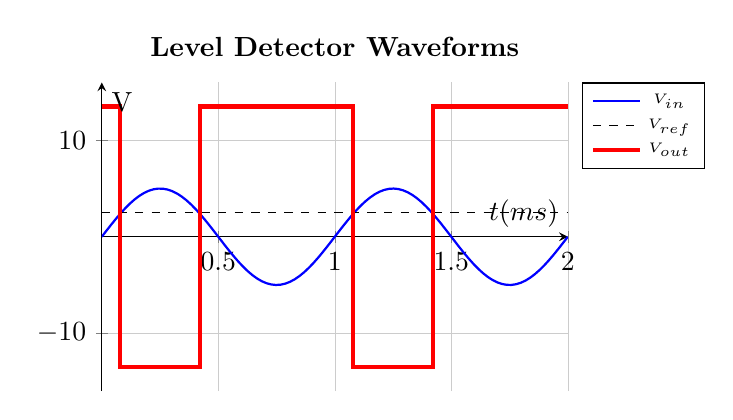
\begin{tikzpicture}
			\begin{axis}[
				axis lines=middle,
				xlabel={$t\text{ (ms)}$},
				ylabel={V},
				xmin=0, xmax=2,
				ymin=-16, ymax=16,
				grid=both,
				grid style={line width=.1pt, draw=gray!20},
				major grid style={line width=.2pt, draw=gray!40},
				width=7.5cm, height=5.5cm,
				title={\textbf{Level Detector Waveforms}},
				legend pos=outer north east,
				legend style={font=\tiny}
				]
				% Input Sine Wave (10Vpp, 1kHz)
				\addplot[thick, blue, domain=0:2, samples=100] {5*sin(deg(2*pi*1*x))};
				\addlegendentry{$V_{in}$}
				
				% Vref line
				\addplot[black,dashed, domain=0:2] {2.5};
				\addlegendentry{$V_{ref}$}				
				% Output Waveform of Inverting Schmitt Trigger
				\addplot[ultra thick, red] coordinates {
					(0, 13.5) (0.078, 13.5) (0.078, -13.5) 
					(0.422, -13.5) (0.422, 13.5) (1.078, 13.5) 
					(1.078, -13.5) (1.422, -13.5) (1.422, 13.5) (2.0, 13.5)
				};
				\addlegendentry{$V_{out}$}
			\end{axis}
		\end{tikzpicture}
		\caption{Input Sine Wave vs Output Rectangular Wave for the Level Detector}
	\end{subfigure}
	\hfill
	\begin{subfigure}[b]{0.38\textwidth}
		\centering
	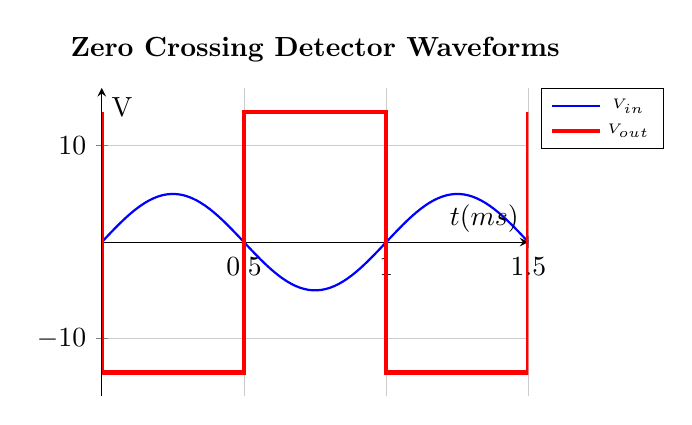
\begin{tikzpicture}
		\begin{axis}[
			axis lines=middle,
			xlabel={$t\text{ (ms)}$},
			ylabel={V},
			xmin=0, xmax=1.5,
			ymin=-16, ymax=16,
			grid=both,
			grid style={line width=.1pt, draw=gray!20},
			major grid style={line width=.2pt, draw=gray!40},
			width=7cm, height=5.5cm,
			title={\textbf{Zero Crossing Detector Waveforms}},
			legend pos=outer north east,
			legend style={font=\tiny}
			]
			% Input Sine Wave (10Vpp, 1kHz)
			\addplot[thick, blue, domain=0:1.5, samples=100] {5*sin(deg(2*pi*1*x))};
			\addlegendentry{$V_{in}$}
			
			% Output Waveform of Inverting Schmitt Trigger
			\addplot[ultra thick, red] coordinates {
				(0, 13.5) (0, 13.5) (0, -13.5) 
				(0.5, -13.5) (0.5, 13.5) (1.0, 13.5) 
				(1.0, -13.5) (1.5, -13.5) (1.5, 13.5)
			};
			\addlegendentry{$V_{out}$}
		\end{axis}
	\end{tikzpicture}
	\caption{Input Sine Wave vs Output Square Wave}
	\end{subfigure}
	\caption{Model waveforms for Inverting voltage comparator and zero crossing detector}
	\label{fig:expected_leveldetector}
\end{figure}


Figure \ref{fig:expected_comparator_graphs} displays the expected time-aligned input/output waveforms and the corresponding X-Y hysteresis loop for the Schmitt trigger circuit.

\begin{figure}[h!]
\centering
\begin{subfigure}[b]{0.58\textwidth}
\centering
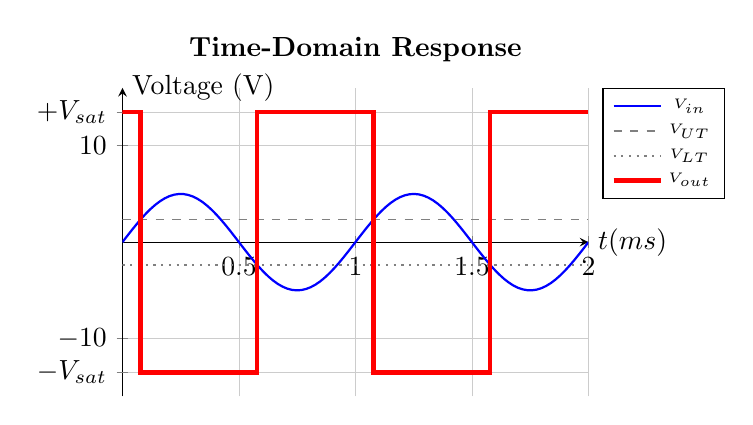
\begin{tikzpicture}
\begin{axis}[
	axis lines=middle,
	xlabel={$t\text{ (ms)}$},
	xlabel style={at={(ticklabel* cs:1)}, anchor=west},
	ylabel={Voltage (V)},
	ylabel style={at={(ticklabel* cs:1)}, anchor=west},
	xmin=0, xmax=2,
	ymin=-16, ymax=16,
	extra y ticks={13.5, -13.5},
	extra y tick labels={$+V_{\text{sat}}$, $-V_{\text{sat}}$},
	grid=both,
	grid style={line width=.1pt, draw=gray!20},
	major grid style={line width=.2pt, draw=gray!40},
	width=7.5cm, height=5.5cm,
	title={\textbf{Time-Domain Response}},
	legend pos=outer north east,
	legend style={font=\tiny}
	]
	% Input Sine Wave (10Vpp, 1kHz)
	\addplot[thick, blue, domain=0:2, samples=100] {5*sin(deg(2*pi*1*x))};
	\addlegendentry{$V_{in}$}	
	% VUT and VLT lines
	\addplot[gray, dashed, domain=0:2] {2.37};
	\addlegendentry{$V_{UT}$}
	\addplot[gray,thick, dotted, domain=0:2] {-2.37};
	\addlegendentry{$V_{LT}$}
	% Output Waveform of Inverting Schmitt Trigger
	\addplot[ultra thick, red] coordinates {
		(0, 13.5) (0.078, 13.5) (0.078, -13.5) 
		(0.578, -13.5) (0.578, 13.5) (1.078, 13.5) 
		(1.078, -13.5) (1.578, -13.5) (1.578, 13.5) (2.0, 13.5)
	};
	\addlegendentry{$V_{out}$};
\end{axis}
\end{tikzpicture}
\caption{Input Sine Wave vs Output Square Wave}
\end{subfigure}
\hfill
\begin{subfigure}[b]{0.38\textwidth}
\centering
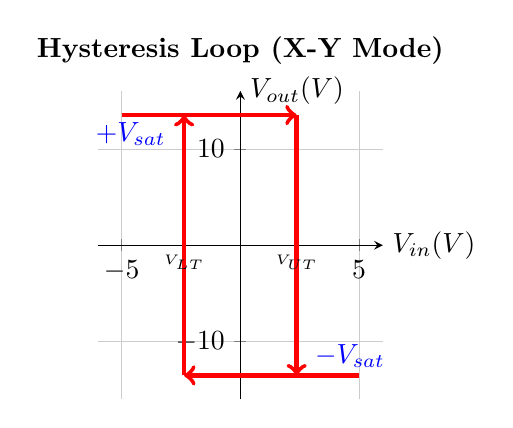
\begin{tikzpicture}
\begin{axis}[
	axis lines=middle,
	xlabel={$V_{in}\text{ (V)}$},
	xlabel style={at={(ticklabel* cs:1)}, anchor=west},
	ylabel={$V_{out}\text{ (V)}$},
	ylabel style={at={(ticklabel* cs:1)}, anchor=west},
	xmin=-6, xmax=6,
	ymin=-16, ymax=16,
	%extra y ticks={13.6, -13.6},
	%extra y tick labels={$+V_{\text{sat}}$, $-V_{\text{sat}}$},
	grid=both,
	grid style={line width=.1pt, draw=gray!20},
	major grid style={line width=.2pt, draw=gray!40},
	width=5.2cm, height=5.5cm,
	title={\textbf{Hysteresis Loop (X-Y Mode)}}
	]
	% Hysteresis loop trajectory
	\draw[ultra thick, red, ->] (axis cs: -5, 13.5) -- (axis cs: 2.37, 13.5);
	\draw[ultra thick, red, ->] (axis cs: 2.37, 13.5) -- (axis cs: 2.37, -13.5);
	\draw[ultra thick, red, ->] (axis cs: 5, -13.5) -- (axis cs: -2.37, -13.5);
	\draw[ultra thick, red, ->] (axis cs: -2.37, -13.5) -- (axis cs: -2.37, 13.5);
	
	% Labels
	\node[font=\tiny, below] at (axis cs: 2.37, 0) {$V_{UT}$};
	\node[font=\tiny, below] at (axis cs: -2.37, 0) {$V_{LT}$};
	\node[anchor= west, blue] at (-6.5, 11.5) {$+V_{\text{sat}}$};
	\node[anchor=east, blue] at (6.5, -11.5) {$-V_{\text{sat}}$};
\end{axis}
\end{tikzpicture}
\caption{Transfer Characteristic Curve}
\end{subfigure}
\caption{Model Graphs and Oscilloscope Display Curves for Inverting Schmitt Trigger}
\label{fig:expected_comparator_graphs}
\end{figure}

\section{Result}
The performance of Open-Loop Comparator and Schmitt Trigger circuits was experimentally evaluated:
\begin{itemize}
\item The zero-crossing and reference voltage detection characteristics of the open-loop comparator were verified.
\item The Inverting Schmitt Trigger thresholds were measured as $V_{UT} = \rule{1.5cm}{0.15mm}\text{ V}$ and $V_{LT} = \rule{1.5cm}{0.15mm}\text{ V}$. % against theoretical values of $+2.37\text{ V}$ and $-2.37\text{ V}$ respectively.
\item The hysteresis width was observed as $V_H = \rule{1.5cm}{0.15mm}\text{ V}$ %(Theoretical: $4.74\text{ V}$, \% Error: \rule{1.2cm}{0.15mm}\%).
\end{itemize}

\section{Questions}
\begin{enumerate}
\item Explain why an open-loop op-amp comparator is highly susceptible to output chatter in the presence of noisy input signals near the reference voltage level.
\item What is the fundamental operational difference between an op-amp used as an amplifier and an op-amp used as a comparator?
\item Why is open-loop voltage gain magnitude ($A_{OL}$) not critical in Schmitt trigger calculations?
\item How can a non-inverting Schmitt trigger circuit be designed, and how do its threshold formulas differ from the inverting topology?
\item How does increasing the feedback resistor $R_2$ affect the hysteresis width $V_H$?
\item What dedicated comparator ICs (e.g., LM311, LM339)\footnote{Refer to the datasheets} offer superior performance over general-purpose op-amps like IC 741 in high-speed digital interfacing applications?
\end{enumerate}